\documentclass[conference]{IEEEtran}

\usepackage{iftex}
\ifXeTeX  % tectonic and other XeTeX builds: IEEEtran's Times through a Unicode clone; pdfLaTeX is unaffected
  \usepackage{fontspec}
  \setmainfont{texgyretermes}[Extension=.otf, UprightFont=*-regular, BoldFont=*-bold, ItalicFont=*-italic,
    BoldItalicFont=*-bolditalic]
  \setmonofont{texgyrecursor}[Extension=.otf, UprightFont=*-regular, BoldFont=*-bold, ItalicFont=*-italic,
    BoldItalicFont=*-bolditalic]
\fi
\usepackage{cite}
\usepackage{amsmath,amssymb}
\usepackage{graphicx}
\usepackage{booktabs}
\usepackage{array}
\PassOptionsToPackage{hyphens}{url}
\usepackage{url}
\usepackage[hidelinks]{hyperref}

\DeclareUrlCommand\code{\urlstyle{tt}}  % code names break like URLs, at / _ - . =
\emergencystretch=1em
\newcommand{\sci}[2]{\ensuremath{#1{\times}10^{#2}}}
\graphicspath{{figures/}}

\begin{document}

\title{Faster but Not Different:\\ Parity-Checked Deployment of the SmolVLA Robot Policy on a Jetson Xavier NX}

\author{\IEEEauthorblockN{Jakhongir Nodirov}
\IEEEauthorblockA{Gachon University, Republic of Korea\\
dil1977@gachon.ac.kr}}

\maketitle

\begin{abstract}
Vision-language-action (VLA) policies are now small enough for embedded GPUs, but compiling one for such hardware can change its actions without raising any error. We deploy SmolVLA, a 450M-parameter VLA policy, on an NVIDIA Jetson Xavier NX and make agreement with the reference implementation a precondition for every speed-up. The policy is exported as three static ONNX graphs (the vision encoder, the VLM prefix and one step of the action expert), its flow-matching loop runs in a C++17 runtime, and every split point is compared with LeRobot's own fp32 tensors, frozen from real LIBERO frames. With TensorRT 8.5, fp32 engines match LeRobot to \sci{1.6}{-5} action standard deviations at 1.0\,s per 50-action chunk. fp16 engines run 3.1 times faster, at 0.33\,s, and stay within 0.060 standard deviations, inside the range of the bf16 precision LeRobot itself runs this checkpoint in. They do so only once every layer the graph types as fp32 is pinned to fp32: TensorRT 8.5's default fp16 build returns finite actions unrelated to the reference. We describe this and four further pitfalls the parity checks exposed, and release the code, measurements and figures.
\end{abstract}

\section{Introduction}

Vision-language-action (VLA) policies map camera images, a task instruction and the robot's state to actions. The first open ones were large: OpenVLA has 7B parameters~\cite{kim2024openvla}, $\pi_0$ about 3B~\cite{black2024pi0}. SmolVLA~\cite{shukor2025smolvla} brings the design down to 450M parameters for affordable hardware: a small vision-language model reads the observation once, and a flow-matching action expert turns noise into a chunk of 50 actions in ten steps.

Running such a policy on the robot means compiling it for an embedded GPU, typically with TensorRT~\cite{nvidia_tensorrt}. Compilation changes the numerics: layers are fused, kernels are chosen by timing, and lower precisions trade range and mantissa for speed. For a policy, changed numbers are changed actions, and some of the changes raise no error at all. A speed-up measured without checking the actions therefore says little. Prior work exports SmolVLA to TensorRT as a single graph and reports a 5.55-fold speed-up over ONNX Runtime's CUDA provider on a data-centre GPU, checked on a synthetic input~\cite{fastcrest2026tether}.

This report deploys SmolVLA on a Jetson Xavier NX, an embedded board that stays on JetPack 5 and TensorRT 8.5, and treats agreement with LeRobot~\cite{cadene2024lerobot}, the reference implementation, as a precondition for any speed-up (Fig.~\ref{fig:pipeline}). Its contributions are:
\begin{itemize}
\item a split of SmolVLA into three static ONNX graphs with an explicit contract, a C++17 runtime that runs the flow-matching loop, and LeRobot's own intermediate tensors as test vectors at every split point (Section~\ref{sec:method});
\item measurements with the real \code{lerobot/smolvla_libero} checkpoint on 16 LIBERO frames: every precision on a CPU, and fp32 and fp16 TensorRT engines on the Jetson (Section~\ref{sec:results});
\item five failure modes the parity checks exposed, four of them silent or misleading, with their fixes (Section~\ref{sec:pitfalls});
\item the code, every measurement as JSON, and the scripts that draw the figures~\cite{smolvlaedge}.
\end{itemize}

\begin{figure*}[t]
\centering
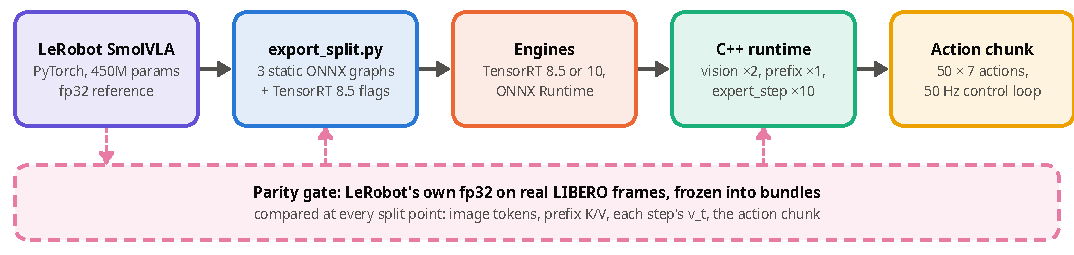
\includegraphics[width=\textwidth]{fig_pipeline}
\caption{The deployment and its parity gate. The policy is exported as three ONNX graphs, built into engines and run by a C++ loop. LeRobot's own fp32 outputs on real frames, frozen into bundles, are compared with the export and the runtime at every split point, not only on the final actions.}
\label{fig:pipeline}
\end{figure*}

\section{Background}

\subsection{SmolVLA}
SmolVLA~\cite{shukor2025smolvla} pairs a SmolVLM-2 backbone~\cite{marafioti2025smolvlm}, truncated to its first 16 layers, with an action expert, a smaller transformer trained with flow matching~\cite{lipman2023flow} in the manner of $\pi_0$~\cite{black2024pi0}. The SigLIP vision encoder~\cite{zhai2023siglip} and a connector turn each camera image into 64 tokens. The VLM layers process the image tokens, the instruction and one state token once per chunk and keep their keys and values. The action expert then integrates from Gaussian noise to a chunk of 50 actions in ten Euler steps, attending to that cache at every step.

\subsection{Precision}
bf16 keeps fp32's exponent range with an 8-bit significand; fp16 has an 11-bit significand but overflows above 65504~\cite{kalamkar2019bf16,micikevicius2018mixed}. Which one a model tolerates depends on its activations, and which one it runs in depends on code as well as on the checkpoint. In LeRobot~0.6.1, a SmolVLA checkpoint saved with \code{load_vlm_weights=true}, as LeRobot's LIBERO training command produces, runs its VLM and action expert in bf16, with the expert's cross-attention keys and values and the small projections in fp32. Its ``fp32'' reference must be built on purpose.

\section{Method}
\label{sec:method}

\subsection{Three graphs and a loop}
Table~\ref{tab:graphs} lists the split. \code{vision} runs once per camera, \code{prefix} once per chunk, and \code{expert_step} ten times (Fig.~\ref{fig:chunk}). Every shape is static and the batch size is one. The Euler loop stays outside the graphs, in the runtime: $x \leftarrow x + \Delta t\, v_t$ with $\Delta t = -0.1$, accumulated in fp32 and rounded as LeRobot rounds it, the product computed separately so that no fused multiply-add changes the result. The graphs are exported to ONNX~\cite{onnx} with \code{torch.onnx} from wrappers around LeRobot's own modules, with three replacements, each tested against LeRobot:
\begin{itemize}
\item a functional K/V cache that returns the concatenated keys and values instead of storing them;
\item the timestep's sinusoidal embedding in fp32 instead of fp64, which TensorRT lacks; its phases reach about 1600~rad, so the phase is reduced exactly modulo one period, which keeps it within \sci{5}{-7} of the fp64 value;
\item the RoPE timescales as a buffer computed by PyTorch, which keeps rotation angles bit-identical to LeRobot's.
\end{itemize}

\begin{table}[t]
\centering
\caption{The three graphs, with \texttt{lerobot/smolvla\_libero}'s shapes}
\label{tab:graphs}
\begin{tabular}{@{}l c >{\raggedright\arraybackslash}p{5.0cm}@{}}
\toprule
Graph & Runs & Inputs $\rightarrow$ outputs \\
\midrule
\code{vision} & 2 & image $3{\times}512{\times}512$ $\rightarrow$ 64 tokens of 960 \\
\code{prefix} & 1 & tokens, 48 token ids and mask, state (32) $\rightarrow$ pad mask (177), K and V of 16 layers, each $5{\times}177{\times}64$ \\
\code{expert_step} & 10 & $x_t$ ($50{\times}32$), $t$, pad mask, K/V $\rightarrow$ $v_t$ ($50{\times}32$) \\
\bottomrule
\end{tabular}
\end{table}

\begin{figure*}[t]
\centering
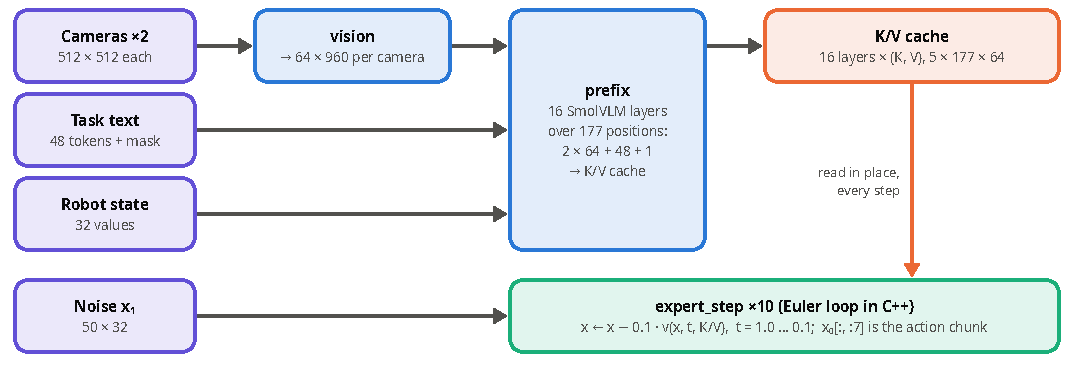
\includegraphics[width=\textwidth]{fig_chunk}
\caption{One action chunk. The prefix covers 177 positions: two cameras' 64 tokens, 48 language tokens and one state token. Its K/V cache is read in place by all ten expert steps. The first 7 of the 32 action dimensions form the chunk.}
\label{fig:chunk}
\end{figure*}

\subsection{The contract and the parity gate}
A manifest records every graph's tensor names, shapes and dtypes, and the runtime refuses graphs that do not match it. A bundle freezes one observation: the preprocessed inputs, the noise, and LeRobot's fp32 tensors at every split point: image tokens, the prefix K/V, $x_t$ and $v_t$ at each step, and the action chunk. Comparing stage by stage tells which graph a fault is in, which the final actions alone do not. The CPU tests require \sci{1}{-5} on the fp32 chunk; the runtime's bench defaults to \sci{1}{-4} on a GPU.

\subsection{The C++ runtime}
The runtime runs one chunk from C++17: \code{vision} per camera, \code{prefix} once, then the Euler loop over \code{expert_step}, with every buffer allocated and bound when it is built and the K/V read in place on the device. One interface has two backends, ONNX Runtime~\cite{onnxruntime} and the TensorRT runtime API of versions 8.5 and 10. A bench checks a chunk against a bundle and times every stage, and a harness runs a 50\,Hz control thread fed by an inference thread.

\subsection{TensorRT 8.5}
TensorRT 10 does not support Volta GPUs and JetPack~6 does not support Xavier, so the board needs graphs for TensorRT 8.5. The exporter's \code{--for-tensorrt85} option lowers the graphs to a real opset 17, writes \code{LayerNormalization}, which TensorRT 8.5 cannot import, as basic operators with fp32 statistics, and, for each fp16 graph, writes the \code{trtexec} flags that pin its fp32 layers (Section~\ref{sec:fp16}).

\section{Experimental setup}
\label{sec:setup}

\textbf{Data.} The \code{lerobot/smolvla_libero} checkpoint (revision \code{a24f1f3}) on 16 frames of the LIBERO~\cite{liu2023libero} dataset it was trained on (\code{lerobot/libero}, revision \code{a1aaacb}): one episode from each of the four LIBERO suites, four frames each, both cameras, the state and the instruction, through the checkpoint's own processors. Each frame has its own noise, shared by every runtime. A synthetic observation adds a seventeenth case on the Jetson.

\textbf{Reference.} LeRobot's \code{predict_action_chunk} in fp32 with TF32 off, on an x86 CPU. Its chunks lie 0.07 standard deviations from the dataset's demonstrated actions over the first ten steps, against 0.72 for the mean action, so weights and preprocessing are right.

\textbf{Metrics.} The largest absolute difference of the normalized $50{\times}7$ chunk, in units of each action dimension's standard deviation; the cosine similarity of the chunk; the relative L2 error of intermediate tensors.

\textbf{Hardware.} A 4-vCPU Xeon virtual machine, one thread, for the CPU study; a Jetson Xavier NX (Volta GPU, JetPack 5.1.6, TensorRT 8.5.2, CUDA 11.4) in its 20\,W six-core mode, clocks not pinned, the GPU at its top 1109\,MHz after each run. Latency is the median (p50) and p99 of 50 chunks after five warm-up chunks.

\section{Results}
\label{sec:results}

\subsection{Random weights}
On a tiny random model with two key/value heads, the split graphs reproduce LeRobot's chunk to \sci{4.8}{-7}, and to \sci{7}{-7} at full SmolVLM2-500M sizes; the C++ runtime is bit-identical to the Python reference. Its 50\,Hz control loop ran 10,000 ticks with no tick left without an action, on a shared virtual machine.

\subsection{Real weights on the CPU}
Table~\ref{tab:cpu} compares every precision with the fp32 reference. The fp32 split graphs agree to \sci{6.3}{-6}. fp16 stays within \sci{2.9}{-3}, while bf16, as LeRobot runs this checkpoint, moves the chunk to 0.049, 4 to 11 times as far as fp16 on the frames where both ran. A probe of every intermediate fp16 tensor found one overflow: the cube $x^3$ of the tanh GELU approximation in the last two SigLIP layers, which tanh's saturation renders harmless where it was checked. Outside it, the largest fp16 values sit 8.5 times below 65504, provided the RMSNorm~\cite{zhang2019rmsnorm} statistics stay in fp32: the VLM's residual stream squared reaches \sci{6.0}{7}.

\begin{table}[t]
\centering
\caption{Real weights on the CPU against LeRobot's fp32: chunk max abs (action std) and smallest cosine, worst frame}
\label{tab:cpu}
\setlength{\tabcolsep}{4pt}
\begin{tabular}{@{}lccc@{}}
\toprule
Variant & Frames & Max abs & Cosine \\
\midrule
Split graphs, fp32 & 16 & \sci{6.3}{-6} & 0.9999999999996 \\
Split graphs, fp16 & 16 & \sci{2.0}{-3} & 0.99999992 \\
PyTorch fp16 (3 layouts) & 4 & \sci{2.9}{-3} & 0.99999975 \\
PyTorch bf16, LeRobot's layout & 16 & \sci{4.9}{-2} & 0.99995 \\
PyTorch bf16, 2 other layouts & 16 & \sci{3.7}{-2} & 0.99996 \\
\bottomrule
\end{tabular}
\end{table}

\subsection{fp32 on the Jetson}
The fp32 engines match LeRobot to \sci{1.6}{-5} on every frame (Table~\ref{tab:jetson}). A chunk takes 1003\,ms, two thirds of it in the vision encoder (Fig.~\ref{fig:latency}). A run peaks at 4.4\,GB of the board's shared memory, and the \code{prefix} engine, whose build asks for a 1\,GiB workspace, built only with the desktop stopped and the file cache dropped.

\begin{figure}[t]
\centering
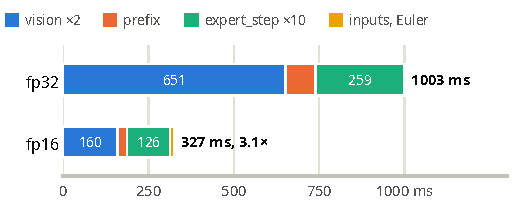
\includegraphics[width=\columnwidth]{fig_latency}
\caption{One action chunk on the Jetson Xavier NX, p50 of each stage on LIBERO frame~0.}
\label{fig:latency}
\end{figure}

\subsection{fp16 on the Jetson}
\label{sec:fp16}
\begin{figure}[t]
\centering
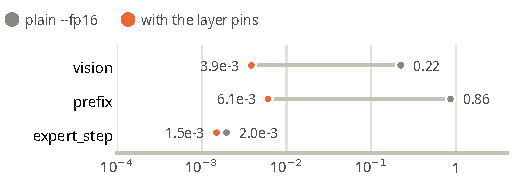
\includegraphics[width=\columnwidth]{fig_pinning}
\caption{Each fp16 engine alone on LeRobot's inputs, relative L2 against fp32, 16 frames.}
\label{fig:pinning}
\end{figure}

\begin{figure*}[t]
\centering
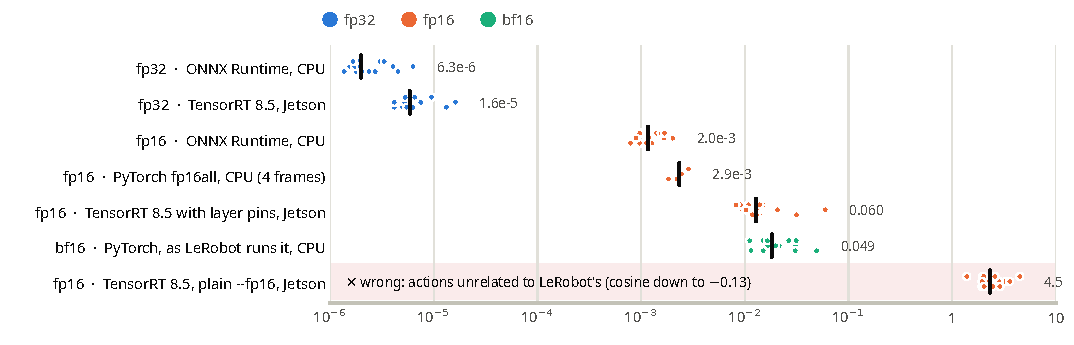
\includegraphics[width=\textwidth]{fig_precision}
\caption{Chunk error against LeRobot's fp32, per LIBERO frame (dots) and median (bar), in action standard deviations. TensorRT fp16 with the layer pins lands with LeRobot's own bf16; without them it is wrong.}
\label{fig:precision}
\end{figure*}

\begin{table*}[t]
\centering
\caption{Failures met during the deployment}
\label{tab:pitfalls}
\begin{tabular}{@{}>{\raggedright\arraybackslash}p{3.1cm}>{\raggedright\arraybackslash}p{5.5cm}>{\raggedright\arraybackslash}p{3.4cm}>{\raggedright\arraybackslash}p{4.8cm}@{}}
\toprule
Failure & Symptom & Caught by & Fix \\
\midrule
1. Weakly typed fp16 & Engines build and run; actions unrelated to LeRobot's (cosine down to $-0.13$) & Per-graph parity on real frames & Pin every fp32-typed layer (\code{trt85_flags}) \\
2. Opset 18 \code{ReduceMean} & Parser ignores the axes input and averages every RMSNorm over all axes; tiny model's chunk off by 0.18, its K/V by 1.1 & Stage-wise parity & Lower to a real opset 17; refuse any other opset \\
3. Myelin \code{Sigmoid} typing & \code{expert_step} fails to build: its fused block holds one fp32 and sixteen fp16 Sigmoids & Build error & Compute every Sigmoid of that graph in fp32 \\
4. Page cache on a Jetson & Third engine fails to load with 1.3\,GB shown available; CUDA memory comes from nvmap, which does not reclaim the page cache & Engine load error with a misleading message & Drop each engine file from the cache once read \\
5. One K/V head in tests & K/V read in the wrong layout gives the same numbers & Two-head test model & Every parity test uses two heads; the injected bug moves the chunk by 0.24 \\
\bottomrule
\end{tabular}
\end{table*}

TensorRT 8.5 has no strongly typed mode. Its ONNX parser marks the layers the graph types as fp16, so a build needs \code{--fp16}, and with that flag the fused kernels of its Myelin backend, which covers nearly each graph whole, evidently compute the graph's fp32 parts in fp16 as well. Each engine alone on LeRobot's inputs then misses by a relative L2 of 0.22 (\code{vision}) and 0.86 (\code{prefix}), and the chunk is unrelated to LeRobot's (Fig.~\ref{fig:pinning}). Pinning every node with an fp32 output to fp32 (\code{--precisionConstraints=obey} with per-layer precisions and output types) brings them to \sci{3.9}{-3} and \sci{6.1}{-3}. \code{expert_step} also needs every Sigmoid in fp32 to build at all (Section~\ref{sec:pitfalls}).

With the pins, the chunk lies within 0.060 of LeRobot's on every frame, 0.013 at the median, with nothing non-finite (Fig.~\ref{fig:precision}). That is the range of LeRobot's own bf16 (median 0.018, worst 0.049), closer to fp32 on 11 of the 16 frames, but 4.3 to 5.6 times as far as PyTorch's fp16 on the frames where both ran. The image tokens and the K/V differ by a similar relative L2 on every frame, between \sci{3.4}{-3} and \sci{5.8}{-3} and between \sci{6.3}{-3} and \sci{7.2}{-3}; what varies is how far the ten Euler steps carry it, up to 0.060 on one frame. Where TensorRT's extra error comes from, kernels or accumulation, was not examined.

A chunk takes 327\,ms, 3.1 times faster than fp32 (timed with the board's desktop stopped; 999\,ms with it running, as for fp16): the vision encoder 4.1 times, the prefix 3.2, an expert step 2.1. Keeping the fp32 parts costs 2.5\% against the unpinned build. A run peaks at 2.7\,GB, and all three engines build with the desktop running.

\begin{table}[t]
\centering
\caption{Real weights on the Jetson Xavier NX, TensorRT 8.5.2}
\label{tab:jetson}
\setlength{\tabcolsep}{3pt}
\begin{tabular}{@{}lcc@{}}
\toprule
 & fp32 & fp16, pinned \\
\midrule
Chunk error, worst (median) & \sci{1.6}{-5} (\sci{5.9}{-6}) & 0.060 (0.013) \\
Chunk cosine, smallest & 0.999999999996 & 0.999975 \\
Image tokens, rel.\ L2 & \sci{1.9}{-6} & \sci{5.8}{-3} \\
Prefix K/V, rel.\ L2 & \sci{2.3}{-6} & \sci{7.2}{-3} \\
$v_t$, 10 steps, rel.\ L2 & \sci{7.1}{-6} & \sci{8.2}{-3} \\
\midrule
Chunk, p50 (p99) & 1003 (1020) ms & 327 (336) ms \\
Vision, prefix, step, p50 & 326 / 88 / 25.9 ms & 80 / 28 / 12.6 ms \\
Peak memory of a run & 4.4 GB & 2.7 GB \\
Engine builds & 65 / 143 / 153 s & 130 / 167 / 170 s \\
\bottomrule
\end{tabular}
\end{table}

\section{Pitfalls the parity checks exposed}
\label{sec:pitfalls}
Table~\ref{tab:pitfalls} lists five failures met on the way. Only the third raised an error.

The first two are the dangerous kind: nothing fails, and the actions are wrong. The first is specific to weakly typed builds, which TensorRT~10 can replace with a strongly typed mode. The second came with a second silent step: \code{torch.onnx}, asked for opset 17, left two of the three graphs at opset 18 and only logged that its converter had failed. The exporter now lowers the graphs itself and refuses any opset other than the one requested.

\section{Limitations}
\label{sec:limits}
Every result is numerical agreement on fixed frames. Whether the fp16 chunks, which sit in bf16's range, change task success in closed loop is not tested; paired simulator rollouts are the next step. The study covers one checkpoint, 16 frames and one board, a Volta-generation Jetson on TensorRT 8.5; the strongly typed TensorRT 10 path is implemented but untested on a GPU. Latency was measured over about a minute, without sustained load or a robot stack sharing the board.

\section{Conclusion}
SmolVLA runs on a Jetson Xavier NX at 0.33\,s per 50-action chunk in fp16, a third of its fp32 time, with actions as close to LeRobot's fp32 as LeRobot's own bf16. Getting there required treating agreement with the reference as a gate at every split point: two of the five failures met along the way produced wrong actions with no error, and only the parity checks found them.

\section*{Acknowledgment}
Parts of the code and of this text were drafted with an AI assistant (Claude, Anthropic) and reviewed by the author, who is responsible for all content.

\bibliographystyle{IEEEtran}
\bibliography{refs}

\end{document}
